% Options for packages loaded elsewhere
\PassOptionsToPackage{unicode}{hyperref}
\PassOptionsToPackage{hyphens}{url}
\PassOptionsToPackage{dvipsnames,svgnames,x11names}{xcolor}
%
\documentclass[
  letterpaper,
  DIV=11,
  numbers=noendperiod]{scrartcl}

\usepackage{amsmath,amssymb}
\usepackage{iftex}
\ifPDFTeX
  \usepackage[T1]{fontenc}
  \usepackage[utf8]{inputenc}
  \usepackage{textcomp} % provide euro and other symbols
\else % if luatex or xetex
  \usepackage{unicode-math}
  \defaultfontfeatures{Scale=MatchLowercase}
  \defaultfontfeatures[\rmfamily]{Ligatures=TeX,Scale=1}
\fi
\usepackage{lmodern}
\ifPDFTeX\else  
    % xetex/luatex font selection
\fi
% Use upquote if available, for straight quotes in verbatim environments
\IfFileExists{upquote.sty}{\usepackage{upquote}}{}
\IfFileExists{microtype.sty}{% use microtype if available
  \usepackage[]{microtype}
  \UseMicrotypeSet[protrusion]{basicmath} % disable protrusion for tt fonts
}{}
\makeatletter
\@ifundefined{KOMAClassName}{% if non-KOMA class
  \IfFileExists{parskip.sty}{%
    \usepackage{parskip}
  }{% else
    \setlength{\parindent}{0pt}
    \setlength{\parskip}{6pt plus 2pt minus 1pt}}
}{% if KOMA class
  \KOMAoptions{parskip=half}}
\makeatother
\usepackage{xcolor}
\setlength{\emergencystretch}{3em} % prevent overfull lines
\setcounter{secnumdepth}{-\maxdimen} % remove section numbering
% Make \paragraph and \subparagraph free-standing
\ifx\paragraph\undefined\else
  \let\oldparagraph\paragraph
  \renewcommand{\paragraph}[1]{\oldparagraph{#1}\mbox{}}
\fi
\ifx\subparagraph\undefined\else
  \let\oldsubparagraph\subparagraph
  \renewcommand{\subparagraph}[1]{\oldsubparagraph{#1}\mbox{}}
\fi

\usepackage{color}
\usepackage{fancyvrb}
\newcommand{\VerbBar}{|}
\newcommand{\VERB}{\Verb[commandchars=\\\{\}]}
\DefineVerbatimEnvironment{Highlighting}{Verbatim}{commandchars=\\\{\}}
% Add ',fontsize=\small' for more characters per line
\usepackage{framed}
\definecolor{shadecolor}{RGB}{241,243,245}
\newenvironment{Shaded}{\begin{snugshade}}{\end{snugshade}}
\newcommand{\AlertTok}[1]{\textcolor[rgb]{0.68,0.00,0.00}{#1}}
\newcommand{\AnnotationTok}[1]{\textcolor[rgb]{0.37,0.37,0.37}{#1}}
\newcommand{\AttributeTok}[1]{\textcolor[rgb]{0.40,0.45,0.13}{#1}}
\newcommand{\BaseNTok}[1]{\textcolor[rgb]{0.68,0.00,0.00}{#1}}
\newcommand{\BuiltInTok}[1]{\textcolor[rgb]{0.00,0.23,0.31}{#1}}
\newcommand{\CharTok}[1]{\textcolor[rgb]{0.13,0.47,0.30}{#1}}
\newcommand{\CommentTok}[1]{\textcolor[rgb]{0.37,0.37,0.37}{#1}}
\newcommand{\CommentVarTok}[1]{\textcolor[rgb]{0.37,0.37,0.37}{\textit{#1}}}
\newcommand{\ConstantTok}[1]{\textcolor[rgb]{0.56,0.35,0.01}{#1}}
\newcommand{\ControlFlowTok}[1]{\textcolor[rgb]{0.00,0.23,0.31}{#1}}
\newcommand{\DataTypeTok}[1]{\textcolor[rgb]{0.68,0.00,0.00}{#1}}
\newcommand{\DecValTok}[1]{\textcolor[rgb]{0.68,0.00,0.00}{#1}}
\newcommand{\DocumentationTok}[1]{\textcolor[rgb]{0.37,0.37,0.37}{\textit{#1}}}
\newcommand{\ErrorTok}[1]{\textcolor[rgb]{0.68,0.00,0.00}{#1}}
\newcommand{\ExtensionTok}[1]{\textcolor[rgb]{0.00,0.23,0.31}{#1}}
\newcommand{\FloatTok}[1]{\textcolor[rgb]{0.68,0.00,0.00}{#1}}
\newcommand{\FunctionTok}[1]{\textcolor[rgb]{0.28,0.35,0.67}{#1}}
\newcommand{\ImportTok}[1]{\textcolor[rgb]{0.00,0.46,0.62}{#1}}
\newcommand{\InformationTok}[1]{\textcolor[rgb]{0.37,0.37,0.37}{#1}}
\newcommand{\KeywordTok}[1]{\textcolor[rgb]{0.00,0.23,0.31}{#1}}
\newcommand{\NormalTok}[1]{\textcolor[rgb]{0.00,0.23,0.31}{#1}}
\newcommand{\OperatorTok}[1]{\textcolor[rgb]{0.37,0.37,0.37}{#1}}
\newcommand{\OtherTok}[1]{\textcolor[rgb]{0.00,0.23,0.31}{#1}}
\newcommand{\PreprocessorTok}[1]{\textcolor[rgb]{0.68,0.00,0.00}{#1}}
\newcommand{\RegionMarkerTok}[1]{\textcolor[rgb]{0.00,0.23,0.31}{#1}}
\newcommand{\SpecialCharTok}[1]{\textcolor[rgb]{0.37,0.37,0.37}{#1}}
\newcommand{\SpecialStringTok}[1]{\textcolor[rgb]{0.13,0.47,0.30}{#1}}
\newcommand{\StringTok}[1]{\textcolor[rgb]{0.13,0.47,0.30}{#1}}
\newcommand{\VariableTok}[1]{\textcolor[rgb]{0.07,0.07,0.07}{#1}}
\newcommand{\VerbatimStringTok}[1]{\textcolor[rgb]{0.13,0.47,0.30}{#1}}
\newcommand{\WarningTok}[1]{\textcolor[rgb]{0.37,0.37,0.37}{\textit{#1}}}

\providecommand{\tightlist}{%
  \setlength{\itemsep}{0pt}\setlength{\parskip}{0pt}}\usepackage{longtable,booktabs,array}
\usepackage{calc} % for calculating minipage widths
% Correct order of tables after \paragraph or \subparagraph
\usepackage{etoolbox}
\makeatletter
\patchcmd\longtable{\par}{\if@noskipsec\mbox{}\fi\par}{}{}
\makeatother
% Allow footnotes in longtable head/foot
\IfFileExists{footnotehyper.sty}{\usepackage{footnotehyper}}{\usepackage{footnote}}
\makesavenoteenv{longtable}
\usepackage{graphicx}
\makeatletter
\def\maxwidth{\ifdim\Gin@nat@width>\linewidth\linewidth\else\Gin@nat@width\fi}
\def\maxheight{\ifdim\Gin@nat@height>\textheight\textheight\else\Gin@nat@height\fi}
\makeatother
% Scale images if necessary, so that they will not overflow the page
% margins by default, and it is still possible to overwrite the defaults
% using explicit options in \includegraphics[width, height, ...]{}
\setkeys{Gin}{width=\maxwidth,height=\maxheight,keepaspectratio}
% Set default figure placement to htbp
\makeatletter
\def\fps@figure{htbp}
\makeatother

\usepackage{fvextra}
\DefineVerbatimEnvironment{Highlighting}{Verbatim}{breaklines,commandchars=\\\{\}}
\KOMAoption{captions}{tableheading}
\makeatletter
\@ifpackageloaded{caption}{}{\usepackage{caption}}
\AtBeginDocument{%
\ifdefined\contentsname
  \renewcommand*\contentsname{Table of contents}
\else
  \newcommand\contentsname{Table of contents}
\fi
\ifdefined\listfigurename
  \renewcommand*\listfigurename{List of Figures}
\else
  \newcommand\listfigurename{List of Figures}
\fi
\ifdefined\listtablename
  \renewcommand*\listtablename{List of Tables}
\else
  \newcommand\listtablename{List of Tables}
\fi
\ifdefined\figurename
  \renewcommand*\figurename{Figure}
\else
  \newcommand\figurename{Figure}
\fi
\ifdefined\tablename
  \renewcommand*\tablename{Table}
\else
  \newcommand\tablename{Table}
\fi
}
\@ifpackageloaded{float}{}{\usepackage{float}}
\floatstyle{ruled}
\@ifundefined{c@chapter}{\newfloat{codelisting}{h}{lop}}{\newfloat{codelisting}{h}{lop}[chapter]}
\floatname{codelisting}{Listing}
\newcommand*\listoflistings{\listof{codelisting}{List of Listings}}
\makeatother
\makeatletter
\@ifpackageloaded{caption}{}{\usepackage{caption}}
\@ifpackageloaded{subcaption}{}{\usepackage{subcaption}}
\makeatother
\makeatletter
\makeatother
\ifLuaTeX
  \usepackage{selnolig}  % disable illegal ligatures
\fi
\IfFileExists{bookmark.sty}{\usepackage{bookmark}}{\usepackage{hyperref}}
\IfFileExists{xurl.sty}{\usepackage{xurl}}{} % add URL line breaks if available
\urlstyle{same} % disable monospaced font for URLs
\hypersetup{
  pdftitle={Homework 1 Solutions},
  colorlinks=true,
  linkcolor={blue},
  filecolor={Maroon},
  citecolor={Blue},
  urlcolor={Blue},
  pdfcreator={LaTeX via pandoc}}

\title{Homework 1 Solutions}
\author{}
\date{}

\begin{document}
\maketitle
\RecustomVerbatimEnvironment{verbatim}{Verbatim}{
showspaces = false,
showtabs = false,
breaksymbolleft={},
breaklines
% Note: setting commandchars=\\\{\} here will cause an error
}

\subsection{Overview}\label{overview}

\subsubsection{Instructions}\label{instructions}

The goal of this homework assignment is to introduce you to
simulation-based data analysis.

\begin{itemize}
\tightlist
\item
  Problem 1 asks you to explore whether a difference between data
  collected from two groups might be statistically meaningful or the
  result of noise. This problem repeats the analysis from
  \href{https://www.youtube.com/watch?v=5Dnw46eC-0o}{Statistics Without
  The Agonizing Pain} by John Rauser (which is a neat watch!).
\item
  Problem 2 asks you to evaluate an interview method for finding the
  level of cheating on a test to determine whether cheating was
  relatively high or low. This problem was adapted from
  \href{https://dataorigami.net/Probabilistic-Programming-and-Bayesian-Methods-for-Hackers/}{Bayesian
  Methods for Hackers}.
\end{itemize}

\subsubsection{Load Environment}\label{load-environment}

The following code loads the environment and makes sure all needed
packages are installed. This should be at the start of most Julia
scripts.

\begin{Shaded}
\begin{Highlighting}[]
\ImportTok{import} \BuiltInTok{Pkg}
\BuiltInTok{Pkg}\NormalTok{.}\FunctionTok{activate}\NormalTok{(}\PreprocessorTok{@\_\_DIR\_\_}\NormalTok{)}
\BuiltInTok{Pkg}\NormalTok{.}\FunctionTok{instantiate}\NormalTok{()}
\end{Highlighting}
\end{Shaded}

The following packages are included in the environment (to help you find
other similar packages in other languages). The code below loads these
packages for use in the subsequent notebook (the desired functionality
for each package is commented next to the package).

\begin{Shaded}
\begin{Highlighting}[]
\ImportTok{using} \BuiltInTok{Random }\CommentTok{\# random number generation and seed{-}setting}
\ImportTok{using} \BuiltInTok{DataFrames }\CommentTok{\# tabular data structure}
\ImportTok{using} \BuiltInTok{CSVFiles }\CommentTok{\# reads/writes .csv files}
\ImportTok{using} \BuiltInTok{Distributions }\CommentTok{\# interface to work with probability distributions}
\ImportTok{using} \BuiltInTok{Plots }\CommentTok{\# plotting library}
\ImportTok{using} \BuiltInTok{StatsBase }\CommentTok{\# adds some basic statistical functionality (means, medians, empirical cumulative densities, etc)}
\ImportTok{using} \BuiltInTok{StatsPlots }\CommentTok{\# for qqplots}
\end{Highlighting}
\end{Shaded}

\subsection{Problems}\label{problems}

\subsubsection{Problem 1}\label{problem-1}

\begin{Shaded}
\begin{Highlighting}[]
\NormalTok{data }\OperatorTok{=} \FunctionTok{DataFrame}\NormalTok{(}\FunctionTok{load}\NormalTok{(}\StringTok{"data/bites.csv"}\NormalTok{)) }\CommentTok{\# load data into DataFrame}

\CommentTok{\# print data variable (semi{-}colon suppresses echoed output in Julia, which in this case would duplicate the output)}
\PreprocessorTok{@show}\NormalTok{ data; }
\end{Highlighting}
\end{Shaded}

\begin{verbatim}
data = 43×2 DataFrame
 Row │ group   bites
     │ String  Int64
─────┼───────────────
   1 │ beer       27
   2 │ beer       20
   3 │ beer       21
   4 │ beer       26
   5 │ beer       27
   6 │ beer       31
   7 │ beer       24
   8 │ beer       21
   9 │ beer       20
  10 │ beer       19
  11 │ beer       23
  12 │ beer       24
  13 │ beer       28
  14 │ beer       19
  15 │ beer       24
  16 │ beer       29
  17 │ beer       18
  18 │ beer       20
  19 │ beer       17
  20 │ beer       31
  21 │ beer       20
  22 │ beer       25
  23 │ beer       28
  24 │ beer       21
  25 │ beer       27
  26 │ water      21
  27 │ water      22
  28 │ water      15
  29 │ water      12
  30 │ water      21
  31 │ water      16
  32 │ water      19
  33 │ water      15
  34 │ water      22
  35 │ water      24
  36 │ water      19
  37 │ water      23
  38 │ water      13
  39 │ water      22
  40 │ water      20
  41 │ water      24
  42 │ water      18
  43 │ water      20
\end{verbatim}

\begin{Shaded}
\begin{Highlighting}[]
\CommentTok{\# split data into vectors of bites for each group}
\NormalTok{beer }\OperatorTok{=}\NormalTok{ data[data.group }\OperatorTok{.==} \StringTok{"beer"}\NormalTok{, }\OperatorTok{:}\NormalTok{bites]}
\NormalTok{water }\OperatorTok{=}\NormalTok{ data[data.group }\OperatorTok{.==} \StringTok{"water"}\NormalTok{, }\OperatorTok{:}\NormalTok{bites]}

\NormalTok{observed\_difference }\OperatorTok{=} \FunctionTok{mean}\NormalTok{(beer) }\OperatorTok{{-}} \FunctionTok{mean}\NormalTok{(water)}
\PreprocessorTok{@show}\NormalTok{ observed\_difference;}
\end{Highlighting}
\end{Shaded}

\begin{verbatim}
observed_difference = 4.37777777777778
\end{verbatim}

\textbf{In this problem}:

\begin{itemize}
\tightlist
\item
  Conduct the above procedure to generate 50,000 simulated datasets
  under the skeptic's hypothesis.
\item
  Plot a histogram of the results and add a dashed vertical line to show
  the experimental difference (if you are using Julia, feel free to look
  at the
  \href{https://viveks.me/simulation-data-analysis/tutorials/julia-plots.html}{Making
  Plots with Julia tutorial} on the class website).
\item
  Draw conclusions about the plausibility of the skeptic's hypothesis
  that there is no difference? Feel free to use any quantitative or
  qualitative assessments of your simulations and the observed
  difference.
\end{itemize}

\textbf{\emph{Solution}}:

First, we write a function (\texttt{simulate\_differences()}) to
generate a new data set and compute the group differences under the
skeptic's hypothesis by shuffling the data across the two groups (this
is called \emph{the non-parametric bootstrap}, which we will talk about
more later):

\begin{Shaded}
\begin{Highlighting}[]
\CommentTok{\# simulate\_differences: function which simulates a new group difference based on the skeptic\textquotesingle{}s hypothesis of no "real" difference between groups by shuffling the input data across groups}
\CommentTok{\# inputs:}
\CommentTok{\#   y₁: vector of bite counts for the beer{-}drinking group}
\CommentTok{\#   y₂: vector of bite counts for the water{-}drinking group}
\CommentTok{\# output:}
\CommentTok{\#   a simulated difference between shuffled group averages}
\KeywordTok{function} \FunctionTok{simulate\_differences}\NormalTok{(y₁, y₂)}
    \CommentTok{\# concatenate both vectors into a single vector}
\NormalTok{    y }\OperatorTok{=} \FunctionTok{vcat}\NormalTok{(y₁, y₂)}

    \CommentTok{\# create new experimental groups consistent with skeptic\textquotesingle{}s hypothesis}
\NormalTok{    y\_shuffle }\OperatorTok{=} \FunctionTok{shuffle}\NormalTok{(y)   }\CommentTok{\# shuffle the combined data}
\NormalTok{    n₁ }\OperatorTok{=} \FunctionTok{length}\NormalTok{(y₁)}
\NormalTok{    x₁ }\OperatorTok{=}\NormalTok{ y\_shuffle[}\FloatTok{1}\OperatorTok{:}\NormalTok{n₁]}
\NormalTok{    x₂ }\OperatorTok{=}\NormalTok{ y\_shuffle[(n₁}\OperatorTok{+}\FloatTok{1}\NormalTok{)}\OperatorTok{:}\KeywordTok{end}\NormalTok{]}

    \CommentTok{\# compute difference between new group means}
\NormalTok{    diff }\OperatorTok{=} \FunctionTok{mean}\NormalTok{(x₁) }\OperatorTok{{-}} \FunctionTok{mean}\NormalTok{(x₂)}
    \ControlFlowTok{return}\NormalTok{ diff}
\KeywordTok{end}
\end{Highlighting}
\end{Shaded}

\begin{verbatim}
simulate_differences (generic function with 1 method)
\end{verbatim}

Next, we evaluate this function 10,000 times and plot the resulting
histogram of differences.

In Julia (and in Python), it is convenient to use a \emph{comprehension}
to automatically allocate the output of the \texttt{for} loop to a
vector. The syntax for a comprehension is
\texttt{{[}some\_function(input)\ for\ input\ in\ some\_range{]}}. In
this case, the index \texttt{input} doesn't appear in the comprehension
as we're just repeating the exact same calculation every time:

\begin{Shaded}
\begin{Highlighting}[]
\NormalTok{shuffled\_differences }\OperatorTok{=}\NormalTok{ [}\FunctionTok{simulate\_differences}\NormalTok{(beer, water) for i }\KeywordTok{in} \FloatTok{1}\OperatorTok{:}\FloatTok{50\_000}\NormalTok{]}
\end{Highlighting}
\end{Shaded}

\begin{verbatim}
50000-element Vector{Float64}:
  0.173333333333332
 -0.7822222222222202
 -0.3999999999999986
  0.9377777777777787
  0.8422222222222224
  0.8422222222222224
  0.36444444444444457
  1.9888888888888907
 -2.884444444444444
 -0.4955555555555584
 -1.7377777777777794
  0.8422222222222224
 -0.9733333333333327
  ⋮
 -0.20888888888888957
  1.5111111111111093
 -0.20888888888888957
 -0.9733333333333327
 -0.3999999999999986
 -2.120000000000001
 -0.4955555555555584
 -0.4955555555555584
  0.9377777777777787
  2.1799999999999997
  1.4155555555555566
 -0.6866666666666674
\end{verbatim}

Without a comprehension, this loop would look something like:

\begin{Shaded}
\begin{Highlighting}[]
\NormalTok{shuffled\_diffs }\OperatorTok{=} \FunctionTok{zeros}\NormalTok{(}\FloatTok{10\_000}\NormalTok{)}
\ControlFlowTok{for}\NormalTok{ i }\KeywordTok{in} \FloatTok{1}\OperatorTok{:}\FunctionTok{length}\NormalTok{(shuffled\_diffs)}
\NormalTok{    shuffled\_differences[i] }\OperatorTok{=} \FunctionTok{simulate\_differences}\NormalTok{(beer, water)}
\ControlFlowTok{end}
\end{Highlighting}
\end{Shaded}

Back to the problem. Now let's plot the histogram. When you see a
\texttt{!} after a function name in Julia, it means that this is a
\emph{mutating function}, which changes the object that it acts on,
rather than returning a new object and preserving the old one. In this
case, the plot object is changed to add new elements to the original
histogram.

\begin{Shaded}
\begin{Highlighting}[]
\NormalTok{hist }\OperatorTok{=} \FunctionTok{histogram}\NormalTok{(shuffled\_differences, label}\OperatorTok{=}\StringTok{"Simulated Differences"}\NormalTok{) }\CommentTok{\# plot the basic histogram}
\CommentTok{\# MAKE SURE TO ADD AXIS LABELS!}
\FunctionTok{xlabel!}\NormalTok{(hist, }\StringTok{"Increased Number of Average Bites for Beer Group"}\NormalTok{)}
\FunctionTok{ylabel!}\NormalTok{(hist, }\StringTok{"Count"}\NormalTok{)}

\CommentTok{\# now add a vertical line for the experimentally{-}observed difference}
\FunctionTok{vline!}\NormalTok{(hist, [observed\_difference], color}\OperatorTok{=:}\NormalTok{red, linestyle}\OperatorTok{=:}\NormalTok{dash, label}\OperatorTok{=}\StringTok{"Observed Difference"}\NormalTok{)}
\end{Highlighting}
\end{Shaded}

\begin{figure}[H]

\centering{

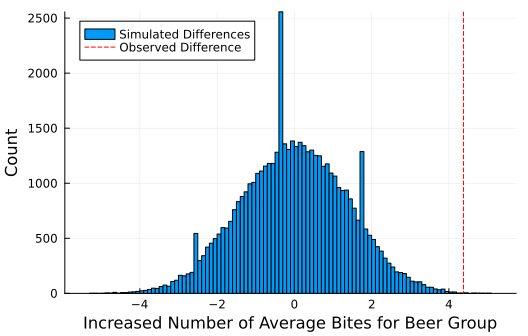
\includegraphics{hw01_files/mediabag/hw01_files/figure-pdf/fig-bites-output-1.pdf}

}

\caption{\label{fig-bites}Histogram of simulated differences between the
average bites for the beer group and the average bites for the water
group under the assumption that differences are due only to random
chance. A positive value indicates that the beer group is bitten more
often. The red line is the group difference from the experimental data.}

\end{figure}%

What do we see from Figure~\ref{fig-bites}?

\begin{itemize}
\item
  The simulated differences follow roughly a normal distribution
  centered at a value of zero. This is not surprising given the
  hypothesis that there is no ``true'' difference in bite frequency
  between the two groups.
\item
  The observed data are extremely unlikely if the skeptic's hypothesis
  is true. We can calculate the probability of seeing data that extreme
  given this hypothesis (also called the \emph{p-value}) by finding the
  empirical cumulative density function of the simulated data vector:

\begin{Shaded}
\begin{Highlighting}[]
\NormalTok{empirical\_cdf }\OperatorTok{=} \FunctionTok{ecdf}\NormalTok{(shuffled\_differences)}
\FloatTok{1} \OperatorTok{{-}} \FunctionTok{empirical\_cdf}\NormalTok{(observed\_difference)}
\end{Highlighting}
\end{Shaded}

\begin{verbatim}
0.00029999999999996696
\end{verbatim}

  This shows that we would only expect, \emph{given the skeptic's
  hypothesis}, to see data at least this extreme by chance in 0.04\% of
  experiments. If we don't think that our experiment is likely to be an
  outlier, this suggests that the skeptic's hypothesis is quite
  unlikely. However, this does not mean our mechanistic theory for the
  group difference is correct: this would require more work and maybe a
  more targeted experiment!
\end{itemize}

\subsubsection{Problem 2}\label{problem-2}

\textbf{In this problem}:

\begin{itemize}
\tightlist
\item
  Derive and code a simulation model for the above interview procedure
  given the ``true'' probability of cheating \(p\).
\item
  Simulate your model (for a class of 100 students) 50,000 times under
  the your hypothesis and the TA's hypothesis, and plot the two
  resulting datasets.
\item
  If you received 31 ``Yes, I cheated'' responses while interviewing
  your class, what could you conclude? Feel free to use any qualitative
  or quantiative assessments to justify your conclusions.
\item
  How useful do you think the interview procedure is to identify
  systemic teaching? What changes to the design might you make?
\end{itemize}

\textbf{\emph{Solution}}:

Let's start by sketching out the simulation model. For every student, we
first need to simulate the outcome of the first coin flip, which has a
50\% probability of heads. If this coin flip comes up as heads, then the
student answers honestly, and admits to cheating with probability \(p\).
If the coin flip comes up tails, the student flips another coin and
answers that they cheated with probability 50\%. After looping over this
procedure for each student in the class, we add up the ``true'' values.

We might code this model as follows.

\begin{Shaded}
\begin{Highlighting}[]
\CommentTok{\# cheating\_model: function which simulates the outcome of the interview procedure described in this problem and returns the number of confessions obtained.}
\CommentTok{\# inputs:}
\CommentTok{\#   p: base probability of cheating under a given hypothesis}
\CommentTok{\#   n: vector of bite counts for the water{-}drinking group}
\CommentTok{\# output:}
\CommentTok{\#   a simulated number of confessions for one realization of the process.}
\KeywordTok{function} \FunctionTok{cheating\_model}\NormalTok{(p, n)}
    \CommentTok{\# initialize the storage vector for whether students admit to cheating}
    \CommentTok{\# we do this with a boolean vector, which is a little faster, but storing integers is basically the same thing}
\NormalTok{    cheat }\OperatorTok{=} \FunctionTok{zeros}\NormalTok{(}\DataTypeTok{Bool}\NormalTok{, n)}
    \CommentTok{\# loop over every student to simulate the interview process}
    \ControlFlowTok{for}\NormalTok{ i }\KeywordTok{in} \FloatTok{1}\OperatorTok{:}\NormalTok{n}
        \CommentTok{\# initial coin flip}
        \CommentTok{\# rand() simulates a uniform random number between 0 and 1}
        \ControlFlowTok{if} \FunctionTok{rand}\NormalTok{() }\OperatorTok{\textgreater{}=} \FloatTok{0.5}
            \CommentTok{\# if this came up heads, simulate whether the student cheated based on the cheating probability}
            \ControlFlowTok{if} \FunctionTok{rand}\NormalTok{() }\OperatorTok{\textless{}}\NormalTok{ p}
\NormalTok{                cheat[i] }\OperatorTok{=} \ConstantTok{true}
            \ControlFlowTok{else}
\NormalTok{                cheat[i] }\OperatorTok{=} \ConstantTok{false}
            \ControlFlowTok{end}
        \ControlFlowTok{else}
            \CommentTok{\# otherwise, simulate another coin flip}
            \ControlFlowTok{if} \FunctionTok{rand}\NormalTok{() }\OperatorTok{\textgreater{}=} \FloatTok{0.5}
\NormalTok{                cheat[i] }\OperatorTok{=} \ConstantTok{true}
            \ControlFlowTok{else}
\NormalTok{                cheat[i] }\OperatorTok{=} \ConstantTok{false}
            \ControlFlowTok{end}
        \ControlFlowTok{end}
    \ControlFlowTok{end}
    \CommentTok{\# return the total number of cheating admissions}
    \ControlFlowTok{return} \FunctionTok{sum}\NormalTok{(cheat)}
\KeywordTok{end}
\end{Highlighting}
\end{Shaded}

\begin{verbatim}
cheating_model (generic function with 1 method)
\end{verbatim}

Now we simulate under our assumption of low cheating and the TA's
assumption of widespread cheating and plot the results.

\begin{Shaded}
\begin{Highlighting}[]
\CommentTok{\# conduct the simulations}
\NormalTok{low\_cheat\_data }\OperatorTok{=}\NormalTok{ [}\FunctionTok{cheating\_model}\NormalTok{(}\FloatTok{0.05}\NormalTok{, }\FloatTok{100}\NormalTok{) for i }\KeywordTok{in} \FloatTok{1}\OperatorTok{:}\FloatTok{50\_000}\NormalTok{]}
\NormalTok{high\_cheat\_data }\OperatorTok{=}\NormalTok{ [}\FunctionTok{cheating\_model}\NormalTok{(}\FloatTok{0.30}\NormalTok{, }\FloatTok{100}\NormalTok{) for i }\KeywordTok{in} \FloatTok{1}\OperatorTok{:}\FloatTok{50\_000}\NormalTok{]}

\CommentTok{\# plot the histograms with axis labels and a vertical line for the "real" outcome of the procedure}
\FunctionTok{histogram}\NormalTok{(low\_cheat\_data, color}\OperatorTok{=:}\NormalTok{blue, label}\OperatorTok{=}\StringTok{"Cheating Rate 5\%"}\NormalTok{, alpha}\OperatorTok{=}\FloatTok{0.4}\NormalTok{)}
\FunctionTok{histogram!}\NormalTok{(high\_cheat\_data, color}\OperatorTok{=:}\NormalTok{red, label}\OperatorTok{=}\StringTok{"Cheating Rate 30\%"}\NormalTok{, alpha}\OperatorTok{=}\FloatTok{0.4}\NormalTok{)}
\FunctionTok{xlabel!}\NormalTok{(}\StringTok{"Number of Students who Confess to Cheating"}\NormalTok{)}
\FunctionTok{ylabel!}\NormalTok{(}\StringTok{"Count"}\NormalTok{)}
\FunctionTok{vline!}\NormalTok{([}\FloatTok{31}\NormalTok{], linestyle}\OperatorTok{=:}\NormalTok{dash, color}\OperatorTok{=:}\NormalTok{green, linewidth}\OperatorTok{=}\FloatTok{3}\NormalTok{, label}\OperatorTok{=}\StringTok{"Observed Outcome"}\NormalTok{)}
\end{Highlighting}
\end{Shaded}

\begin{figure}[H]

\centering{

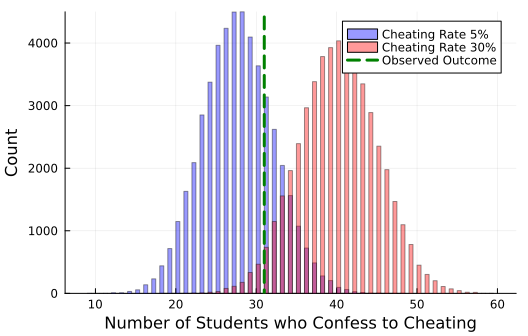
\includegraphics{hw01_files/mediabag/hw01_files/figure-pdf/fig-cheating-output-1.pdf}

}

\caption{\label{fig-cheating}Histograms of the number of simulated
confessions obtained under the hypothesis of a 5\% cheating rate (blue)
and a 30\% cheating rate (red). The green line is the observed number of
cheating confessions.}

\end{figure}%

From Figure~\ref{fig-cheating}, we can see:

\begin{itemize}
\item
  The distributions look roughly normal (not surprising given the
  Central Limit Theorem!).
\item
  There is some overlap around the 25-42 confession count rate. Lower
  than 25 students confessing would strongly suggest that the TA is
  overstating the rate of cheating, while more than 40 would strongly
  suggest that we are underestimating the cheating rate.
\item
  Note that neither of these is ``confirmation'' of either theory, but
  evidence about the relative proportion of cheating being more or less
  consistent with one of our hypotheses.
\item
  The outcome of 31 confessions is in the range where the evidence isn't
  completely clear either way. However, it appears more likely that this
  outcome is explained by a lower rate of cheating than a higher rate.
  For example, under our hypothesis, the ``high-tail'' p-value of the
  outcome is:

\begin{Shaded}
\begin{Highlighting}[]
\NormalTok{ecdf\_low }\OperatorTok{=} \FunctionTok{ecdf}\NormalTok{(low\_cheat\_data)}
\FloatTok{1} \OperatorTok{{-}} \FunctionTok{ecdf\_low}\NormalTok{(}\FloatTok{31}\NormalTok{)}
\end{Highlighting}
\end{Shaded}

\begin{verbatim}
0.18416
\end{verbatim}

  while under the TA's hypothesis, the ``low-tail'' p-value is

\begin{Shaded}
\begin{Highlighting}[]
\NormalTok{ecdf\_high }\OperatorTok{=} \FunctionTok{ecdf}\NormalTok{(high\_cheat\_data)}
\FunctionTok{ecdf\_high}\NormalTok{(}\FloatTok{31}\NormalTok{)}
\end{Highlighting}
\end{Shaded}

\begin{verbatim}
0.03932
\end{verbatim}

  So there is a 18\% probability of seeing 31 or more confessions under
  our assumed 5\% cheating rate, while there is only a 4\% probability
  of seeing 31 or fewer confessions under the TA's assumed 30\% cheating
  rate, which seems to suggest a lower rate is more likely.
\item
  We can't draw any strong conclusions from this, but we will talk more
  later this semester about how to quantify consistency of models with
  data based on simulations!
\item
  This interview process is noisy, but appears to work to separate very
  large differences in cheating rates. On the other hand, it might not
  work so well if we cared about the difference between 5\% cheating and
  10\% cheating rates, as the difference in the ``true'' confessions
  would be swamped by the coin flips. If we wanted to tease out those
  differences, we could use a weighted coin (to increase the number of
  ``honest'' confessions).
\end{itemize}

Later in the semester, we will look at methods for how we might quantify
what base cheating rates are consistent with a given outcome (though we
won't apply them to this example!).

\subsection{Problem 3}\label{problem-3}

\textbf{In this problem}:

\begin{itemize}
\tightlist
\item
  Write a function \texttt{galton\_sim} which simulates \texttt{n}
  Galton board trials (assume the board has 8 board rows, as in the
  image above) and returns a vector with the number of balls which fall
  into each bin. You can assume (for now) that the board is fair,
  \emph{e.g.} that the probability of a left or right bounce is 0.5; you
  may want to make this probability a function parameter so you can
  change it later.
\item
  Run your simulation for a sample of 50 balls. Create a histogram of
  the results, with each bar corresponding to one bin. Make sure you use
  a random seed for reproducibility, and label your axes!
\item
  Each Galton board trial can be represented as a realization from a
  \href{https://en.wikipedia.org/wiki/Binomial_distribution}{binomial
  distribution}. But as we noted above, by the Central Limit Theorem,
  the distribution of a large enough number of trials should be
  approximately normal. Use a
  \href{https://en.wikipedia.org/wiki/Q\%E2\%80\%93Q_plot}{quantile-quantile
  (Q-Q) plot} to compare a fitted normal distribution with your
  simulation results. How well does a normal distribution fit the data?
\item
  Repeat your simulation experiment with 250 trials and compare to a
  normal distribution. Does it describe the empirical distribution
  better?
\item
  If the probability of a left bounce is 70\%, what does this do to the
  fit of a normal distribution? What other distribution might you use if
  not a normal and why?
\end{itemize}

\textbf{\emph{Solution}}:

First, we write the \texttt{galton\_sim} function.

\begin{Shaded}
\begin{Highlighting}[]
\CommentTok{\# p is the probability of a left bounce}
\KeywordTok{function} \FunctionTok{galton\_sim}\NormalTok{(n\_balls, n\_rows; p}\OperatorTok{=}\FloatTok{0.5}\NormalTok{)}
\NormalTok{    n\_bins }\OperatorTok{=}\NormalTok{ n\_rows }\OperatorTok{+} \FloatTok{1} \CommentTok{\# number of bins balls can fall into}
    \CommentTok{\# this subfunction simulates the trajectory of a single ball; this is not entirely necessary but cleans things up a bit}
    \KeywordTok{function} \FunctionTok{simulate\_ball}\NormalTok{(n\_rows, p)}
\NormalTok{        bin }\OperatorTok{=} \FloatTok{0} \CommentTok{\# start in the center}
        \CommentTok{\# for every row, see if the ball bounces to the left (0) or to the right (+1)}
        \CommentTok{\# the accounting here is a little different than might be intuitive: it\textquotesingle{}s easier to calculate the bin if we start from 0 (all left bounces) and just count the number of right increments. We could also have set this up to start in the middle and bounce to the left/right with {-}/+ 1.}
        \ControlFlowTok{for}\NormalTok{ row }\KeywordTok{in} \FloatTok{1}\OperatorTok{:}\NormalTok{n\_rows}
\NormalTok{            bin }\OperatorTok{=}\NormalTok{ bin }\OperatorTok{+} \FunctionTok{sample}\NormalTok{([}\FloatTok{0}\NormalTok{, }\FloatTok{1}\NormalTok{], }\FunctionTok{ProbabilityWeights}\NormalTok{([p, }\FloatTok{1}\OperatorTok{{-}}\NormalTok{p]))  }\CommentTok{\# prob}
        \ControlFlowTok{end}
        \ControlFlowTok{return}\NormalTok{ bin}
    \KeywordTok{end}
    \CommentTok{\# simulate outcome for every ball}
    \CommentTok{\# the use of a comprehension lets us avoid pre{-}allocation and looping}
\NormalTok{    bins }\OperatorTok{=}\NormalTok{ [}\FunctionTok{simulate\_ball}\NormalTok{(n\_rows, p) for \_ }\KeywordTok{in} \FloatTok{1}\OperatorTok{:}\NormalTok{n\_balls] }\CommentTok{\# the \_ just avoids introducing a new counter variable we don\textquotesingle{}t use}

    \ControlFlowTok{return}\NormalTok{ bins }\CommentTok{\# return simulated outcomes}
\KeywordTok{end}
\end{Highlighting}
\end{Shaded}

Next, we run our simulation for 50 balls and create a histogram.

\begin{Shaded}
\begin{Highlighting}[]
\BuiltInTok{Random}\NormalTok{.}\FunctionTok{seed!}\NormalTok{(}\FloatTok{1}\NormalTok{)}

\NormalTok{galton\_simulation }\OperatorTok{=} \FunctionTok{galton\_sim}\NormalTok{(}\FloatTok{50}\NormalTok{, }\FloatTok{8}\NormalTok{)}
\FunctionTok{histogram}\NormalTok{(galton\_simulation, legend}\OperatorTok{=:}\ConstantTok{false}\NormalTok{) }\CommentTok{\# plot histogram}
\FunctionTok{xlabel!}\NormalTok{(}\StringTok{"Galton Board Bin"}\NormalTok{)}
\FunctionTok{ylabel!}\NormalTok{(}\StringTok{"Ball Count"}\NormalTok{)}
\end{Highlighting}
\end{Shaded}

\begin{figure}[H]

{\centering 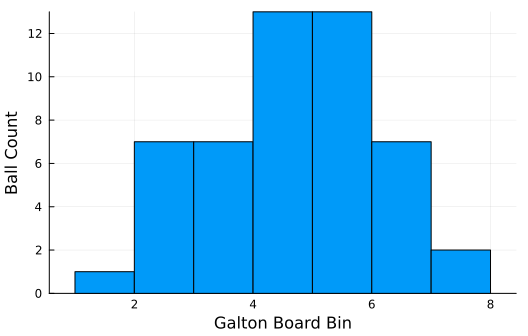
\includegraphics{hw01_files/mediabag/hw01_files/figure-pdf/cell-15-output-1.pdf}

}

\caption{50 Ball Galton Board Histogram}

\end{figure}%

How well does a normal distribution fit this data? We use
\texttt{StatsPlots.qqplot()} to check.

\begin{Shaded}
\begin{Highlighting}[]
\FunctionTok{qqplot}\NormalTok{(Normal, galton\_simulation)}
\FunctionTok{xlabel!}\NormalTok{(}\StringTok{"Theoretical Normal Quantiles"}\NormalTok{)}
\FunctionTok{ylabel!}\NormalTok{(}\StringTok{"Empirical Quantiles"}\NormalTok{)}
\end{Highlighting}
\end{Shaded}

\begin{figure}[H]

\centering{

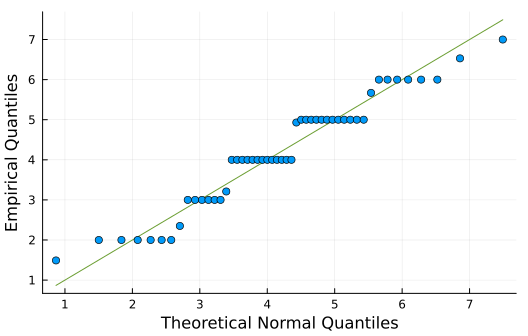
\includegraphics{hw01_files/mediabag/hw01_files/figure-pdf/fig-galton-qq-1-output-1.pdf}

}

\caption{\label{fig-galton-qq-1}50 Ball Galton Board QQ Plot}

\end{figure}%

Figure~\ref{fig-galton-qq-1} might be slightly tricky to interpret as
the data is not continuous. We can see how the repeated samples form
horizontal lines across the 1-1 line. But in general, the fit is pretty
good; the values seem to follow those predicted by a normal once you
account for the discretization.

Let's repeat this with 250 samples:

\begin{Shaded}
\begin{Highlighting}[]
\NormalTok{galton\_simulation }\OperatorTok{=} \FunctionTok{galton\_sim}\NormalTok{(}\FloatTok{250}\NormalTok{, }\FloatTok{8}\NormalTok{)}
\FunctionTok{histogram}\NormalTok{(galton\_simulation, legend}\OperatorTok{=:}\ConstantTok{false}\NormalTok{) }\CommentTok{\# plot histogram}
\FunctionTok{xlabel!}\NormalTok{(}\StringTok{"Galton Board Bin"}\NormalTok{)}
\FunctionTok{ylabel!}\NormalTok{(}\StringTok{"Ball Count"}\NormalTok{)}
\end{Highlighting}
\end{Shaded}

\begin{figure}[H]

{\centering 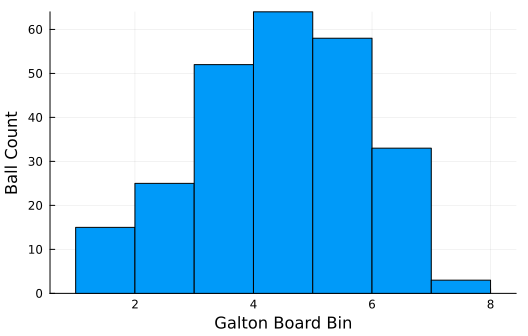
\includegraphics{hw01_files/mediabag/hw01_files/figure-pdf/cell-17-output-1.pdf}

}

\caption{250 Ball Galton Board Histogram}

\end{figure}%

\begin{Shaded}
\begin{Highlighting}[]
\FunctionTok{qqplot}\NormalTok{(Normal, galton\_simulation)}
\FunctionTok{xlabel!}\NormalTok{(}\StringTok{"Theoretical Normal Quantiles"}\NormalTok{)}
\FunctionTok{ylabel!}\NormalTok{(}\StringTok{"Empirical Quantiles"}\NormalTok{)}
\end{Highlighting}
\end{Shaded}

\begin{figure}[H]

\centering{

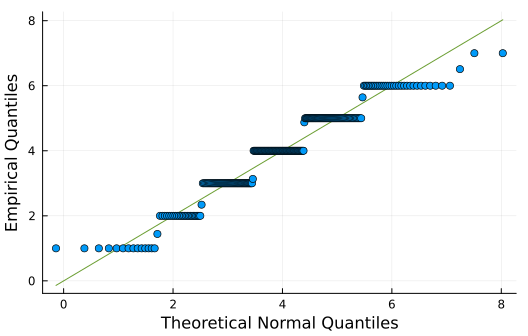
\includegraphics{hw01_files/mediabag/hw01_files/figure-pdf/fig-galton-qq-2-output-1.pdf}

}

\caption{\label{fig-galton-qq-2}250 Ball Galton Board QQ Plot}

\end{figure}%

Figure~\ref{fig-galton-qq-2} is similar to the last 50-ball simulation,
which is not entirely surprising given that the Central Limit Theorem
should only work better with larger samples.

Finally, let's test with a 70\% probability of a left bounce.

\begin{Shaded}
\begin{Highlighting}[]
\NormalTok{galton\_simulation }\OperatorTok{=} \FunctionTok{galton\_sim}\NormalTok{(}\FloatTok{250}\NormalTok{, }\FloatTok{8}\NormalTok{, p}\OperatorTok{=}\FloatTok{0.7}\NormalTok{)}
\FunctionTok{histogram}\NormalTok{(galton\_simulation, legend}\OperatorTok{=:}\ConstantTok{false}\NormalTok{) }\CommentTok{\# plot histogram}
\FunctionTok{xlabel!}\NormalTok{(}\StringTok{"Galton Board Bin"}\NormalTok{)}
\FunctionTok{ylabel!}\NormalTok{(}\StringTok{"Ball Count"}\NormalTok{)}
\end{Highlighting}
\end{Shaded}

\begin{figure}[H]

\centering{

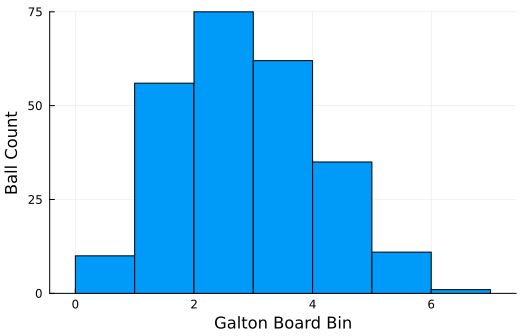
\includegraphics{hw01_files/mediabag/hw01_files/figure-pdf/fig-galton-hist-skewed-output-1.pdf}

}

\caption{\label{fig-galton-hist-skewed}Histogram for Galton Board with
70\% left bounce.}

\end{figure}%

\begin{Shaded}
\begin{Highlighting}[]
\FunctionTok{qqplot}\NormalTok{(Normal, galton\_simulation)}
\FunctionTok{xlabel!}\NormalTok{(}\StringTok{"Theoretical Normal Quantiles"}\NormalTok{)}
\FunctionTok{ylabel!}\NormalTok{(}\StringTok{"Empirical Quantiles"}\NormalTok{)}
\end{Highlighting}
\end{Shaded}

\begin{figure}[H]

\centering{

\includegraphics{hw01_files/mediabag/hw01_files/figure-pdf/fig-galton-qq-3-output-1.pdf}

}

\caption{\label{fig-galton-qq-3}QQ plot for Galton Board with 70\% left
bounce.}

\end{figure}%

We can see a bit more of a skew in Figure~\ref{fig-galton-hist-skewed},
though Figure~\ref{fig-galton-qq-3} still looks reasonable. We could
think about using a SkewNormal distribution to capture that skew.

\subsection{Problem 4}\label{problem-4}

\textbf{In this problem}:

\begin{itemize}
\tightlist
\item
  Write down a model which encodes the Showcase rules as a function of
  the showcase value and your bid. You can assume that your wagering is
  independent of your opponent.
\item
  Select and fit a distribution to the above statistics (you have some
  freedom to pick a distribution, but make sure you justify it).
\item
  Using 1,000 samples from your price distribution in your model, plot
  the expected winnings for bids from \$20,000 through \$72,000.
\item
  Find the bid which maximizes your expected winnings. If you were
  playing \emph{The Price Is Right}, is this the strategy you would
  adopt, or are there other considerations you would take into account
  which were not included in this model?
\end{itemize}

\textbf{\emph{Solution}}:

Here's a function for the outcome of a bid:

\begin{Shaded}
\begin{Highlighting}[]
\KeywordTok{function} \FunctionTok{showcase\_model}\NormalTok{(value, bid)}
    \ControlFlowTok{if}\NormalTok{ bid }\OperatorTok{\textgreater{}}\NormalTok{ value}
\NormalTok{        winnings }\OperatorTok{=} \FloatTok{0}
    \ControlFlowTok{elseif}\NormalTok{ value }\OperatorTok{{-}}\NormalTok{ bid }\OperatorTok{\textless{}} \FloatTok{250}
\NormalTok{        winnings }\OperatorTok{=} \FloatTok{2} \OperatorTok{*}\NormalTok{ value}
    \ControlFlowTok{else}
\NormalTok{        winnings }\OperatorTok{=}\NormalTok{ value}
    \ControlFlowTok{end}
    \ControlFlowTok{return}\NormalTok{ winnings}
\KeywordTok{end}
\end{Highlighting}
\end{Shaded}

\begin{verbatim}
showcase_model (generic function with 1 method)
\end{verbatim}

We'll use a truncated normal distribution to reflect an assumption that
moderate showcase values (near the median) are more typical than the
extremes (this is an assumption, not part of the problem; other choices
are fine!).

\begin{Shaded}
\begin{Highlighting}[]
\NormalTok{showcase\_dist }\OperatorTok{=} \FunctionTok{truncated}\NormalTok{(}\FunctionTok{Normal}\NormalTok{(}\FloatTok{33\_048}\NormalTok{, }\FloatTok{5\_000}\NormalTok{); lower}\OperatorTok{=}\FloatTok{20\_432}\NormalTok{, upper}\OperatorTok{=}\FloatTok{72\_409}\NormalTok{)}
\FunctionTok{histogram}\NormalTok{(}\FunctionTok{rand}\NormalTok{(showcase\_dist, }\FloatTok{100\_000}\NormalTok{))}
\end{Highlighting}
\end{Shaded}

\begin{figure}[H]

\centering{

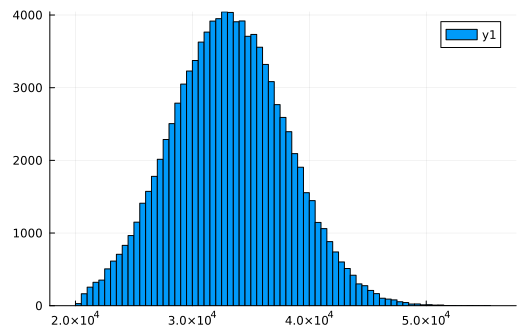
\includegraphics{hw01_files/mediabag/hw01_files/figure-pdf/cell-22-output-1.pdf}

}

\end{figure}%

Now let's write a function to calculate the expected winnings for a
given bid, which we will then evaluate through the bidding range.

\begin{Shaded}
\begin{Highlighting}[]
\KeywordTok{function} \FunctionTok{showcase\_winnings}\NormalTok{(bid, value\_dist)}
    \CommentTok{\# sample 100,000 values of showcases}
\NormalTok{    showcase\_values }\OperatorTok{=} \FunctionTok{rand}\NormalTok{(value\_dist, }\FloatTok{100\_000}\NormalTok{)}
\NormalTok{    winnings }\OperatorTok{=}\NormalTok{ [}\FunctionTok{showcase\_model}\NormalTok{(val, bid) for val }\KeywordTok{in}\NormalTok{ showcase\_values]}
    \ControlFlowTok{return} \FunctionTok{mean}\NormalTok{(winnings)}
\KeywordTok{end}

\NormalTok{bids }\OperatorTok{=} \FloatTok{20\_000}\OperatorTok{:}\FloatTok{1\_000}\OperatorTok{:}\FloatTok{72\_000}
\NormalTok{exp\_winnings }\OperatorTok{=}\NormalTok{ [}\FunctionTok{showcase\_winnings}\NormalTok{(bid, showcase\_dist) for bid }\KeywordTok{in}\NormalTok{ bids]}
\FunctionTok{plot}\NormalTok{(bids, exp\_winnings)}
\end{Highlighting}
\end{Shaded}

\begin{figure}[H]

\centering{

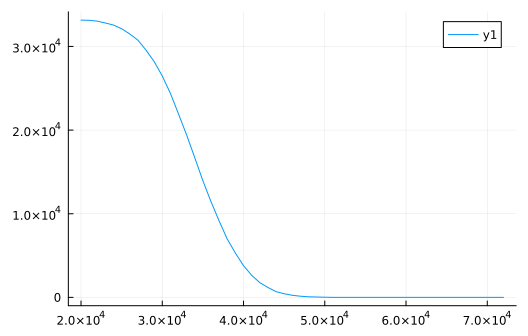
\includegraphics{hw01_files/mediabag/hw01_files/figure-pdf/fig-expected-winnings-output-1.pdf}

}

\end{figure}%

\begin{Shaded}
\begin{Highlighting}[]
\NormalTok{bids[}\FunctionTok{argmax}\NormalTok{(exp\_winnings)]}
\end{Highlighting}
\end{Shaded}

\begin{verbatim}
20000
\end{verbatim}

So with this assumed distribution, the lowest bid maximizes the expected
winnings because there is a large skew to the showcase values, meaning
that higher bids pose a correspondingly higher probability of
overbidding. This would likely not translate well to the actual show
given that the lowest bid also increases the probability of being outbid
by the opponent. We also might have actual clues from the showcase
itself about the relative value within the distribution, rather than
assuming that it's random.



\end{document}
